\documentclass{standalone}
\usepackage{tikz}
\usetikzlibrary{patterns, positioning}
\usepackage[sfdefault]{ClearSans} %% option 'sfdefault' activates Clear Sans as the default text font
\usepackage[T1]{fontenc}

\begin{document}
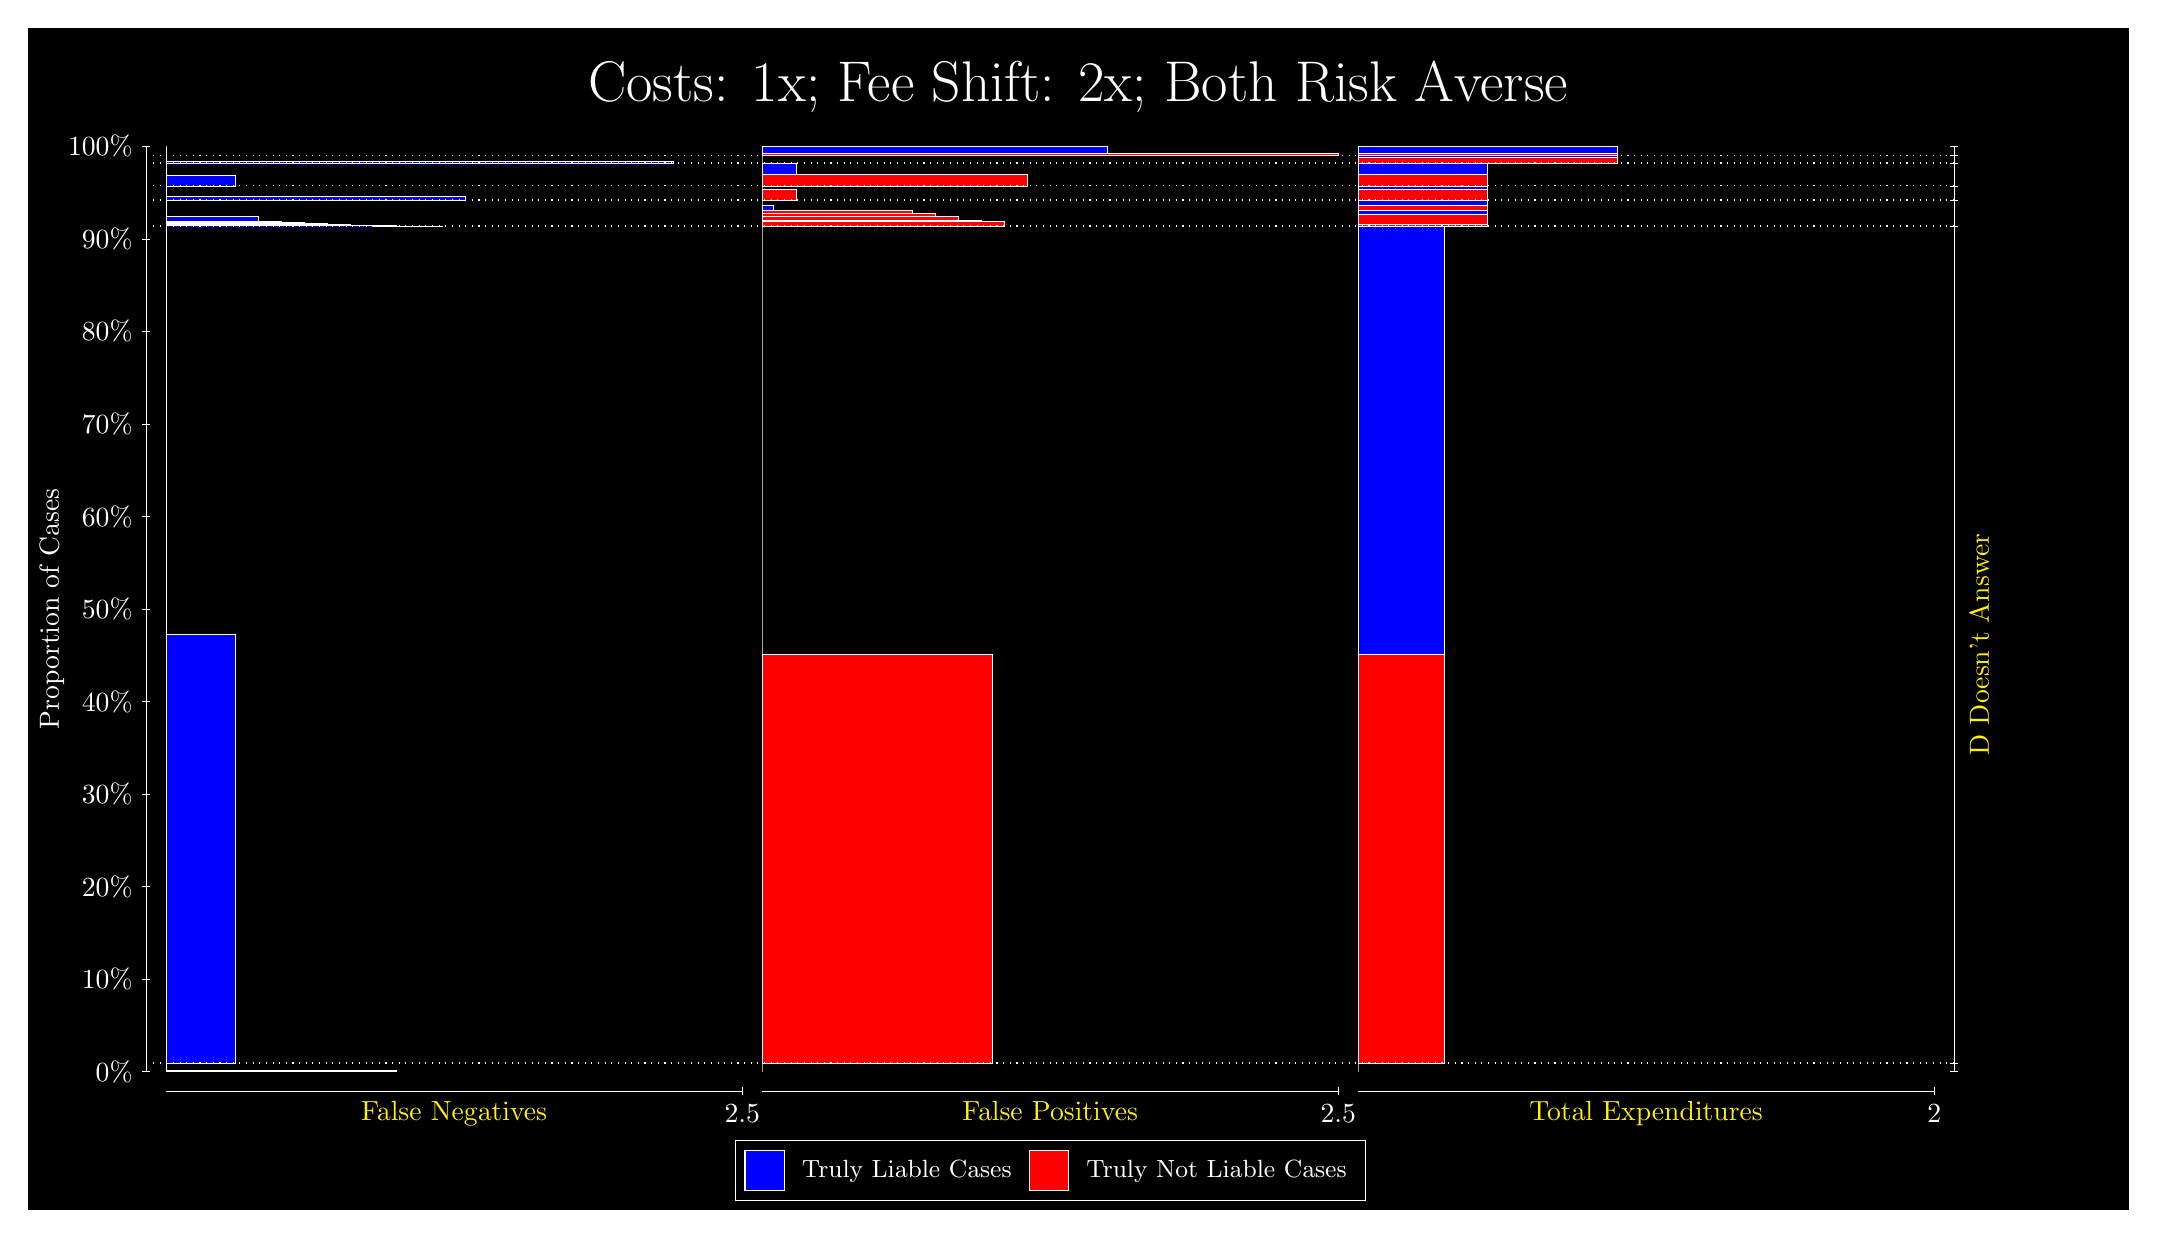
\begin{tikzpicture}
\draw[fill=black] (0,0) rectangle (26.667,15);
\draw[text=white] (0,13.5) rectangle (26.667,15) node[midway] {\huge Costs: 1x; Fee Shift: 2x; Both Risk Averse};
\draw[white, very thin] (1.5,1.75) -- (1.5,13.5);
\node[rotate=90, text=white, anchor=center] at (0.3, 7.625) {Proportion of Cases};
\draw[white, very thin] (1.45,1.75) -- (1.55,1.75);
\node[text=white, anchor=east] at (1.45, 1.75) {0\%};
\draw[white, very thin] (1.45,2.925) -- (1.55,2.925);
\node[text=white, anchor=east] at (1.45, 2.925) {10\%};
\draw[white, very thin] (1.45,4.1) -- (1.55,4.1);
\node[text=white, anchor=east] at (1.45, 4.1) {20\%};
\draw[white, very thin] (1.45,5.275) -- (1.55,5.275);
\node[text=white, anchor=east] at (1.45, 5.275) {30\%};
\draw[white, very thin] (1.45,6.45) -- (1.55,6.45);
\node[text=white, anchor=east] at (1.45, 6.45) {40\%};
\draw[white, very thin] (1.45,7.625) -- (1.55,7.625);
\node[text=white, anchor=east] at (1.45, 7.625) {50\%};
\draw[white, very thin] (1.45,8.8) -- (1.55,8.8);
\node[text=white, anchor=east] at (1.45, 8.8) {60\%};
\draw[white, very thin] (1.45,9.975) -- (1.55,9.975);
\node[text=white, anchor=east] at (1.45, 9.975) {70\%};
\draw[white, very thin] (1.45,11.15) -- (1.55,11.15);
\node[text=white, anchor=east] at (1.45, 11.15) {80\%};
\draw[white, very thin] (1.45,12.325) -- (1.55,12.325);
\node[text=white, anchor=east] at (1.45, 12.325) {90\%};
\draw[white, very thin] (1.45,13.5) -- (1.55,13.5);
\node[text=white, anchor=east] at (1.45, 13.5) {100\%};

\draw[white, very thin] (24.457,1.75) -- (24.457,13.5);
\draw[white, very thin] (24.407,1.75) -- (24.507,1.75);
\node[anchor=west] at (24.407, 1.75) {};
\draw[white, very thin] (24.407,1.8589) -- (24.507,1.8589);
\node[anchor=west] at (24.407, 1.8589) {};
\draw[white, very thin] (24.407,12.488) -- (24.507,12.488);
\node[anchor=west] at (24.407, 12.488) {};
\draw[white, very thin] (24.407,12.818) -- (24.507,12.818);
\node[anchor=west] at (24.407, 12.818) {};
\draw[white, very thin] (24.407,12.997) -- (24.507,12.997);
\node[anchor=west] at (24.407, 12.997) {};
\draw[white, very thin] (24.407,13.288) -- (24.507,13.288);
\node[anchor=west] at (24.407, 13.288) {};
\draw[white, very thin] (24.407,13.386) -- (24.507,13.386);
\node[anchor=west] at (24.407, 13.386) {};
\draw[white, very thin] (24.407,13.5) -- (24.507,13.5);
\node[anchor=west] at (24.407, 13.5) {};

\draw[white, very thin, fill=blue] (1.75,1.75) rectangle (4.6775,1.7615);
\draw[white, very thin, fill=red] (1.75,1.7615) rectangle (1.75,1.8589);
\draw[white, very thin, fill=blue] (1.75,1.8589) rectangle (2.6283,7.2972);
\draw[white, very thin, fill=red] (1.75,7.2972) rectangle (1.75,12.488);
\draw[white, very thin, fill=blue] (1.75,12.488) rectangle (5.2631,12.489);
\draw[white, very thin, fill=blue] (1.75,12.489) rectangle (4.9703,12.49);
\draw[white, very thin, fill=blue] (1.75,12.49) rectangle (4.6775,12.492);
\draw[white, very thin, fill=blue] (1.75,12.492) rectangle (4.3848,12.492);
\draw[white, very thin, fill=blue] (1.75,12.492) rectangle (4.3848,12.493);
\draw[white, very thin, fill=blue] (1.75,12.493) rectangle (4.092,12.506);
\draw[white, very thin, fill=blue] (1.75,12.506) rectangle (3.7993,12.519);
\draw[white, very thin, fill=blue] (1.75,12.519) rectangle (3.5065,12.541);
\draw[white, very thin, fill=blue] (1.75,12.541) rectangle (3.2138,12.552);
\draw[white, very thin, fill=blue] (1.75,12.552) rectangle (2.921,12.614);
\draw[white, very thin, fill=red] (1.75,12.614) rectangle (1.75,12.818);
\draw[white, very thin, fill=blue] (1.75,12.818) rectangle (5.5558,12.866);
\draw[white, very thin, fill=red] (1.75,12.866) rectangle (1.75,12.997);
\draw[white, very thin, fill=blue] (1.75,12.997) rectangle (2.6283,13.135);
\draw[white, very thin, fill=red] (1.75,13.135) rectangle (1.75,13.288);
\draw[white, very thin, fill=blue] (1.75,13.288) rectangle (8.1906,13.309);
\draw[white, very thin, fill=red] (1.75,13.309) rectangle (1.75,13.386);
\draw[white, very thin, fill=red] (1.75,13.386) rectangle (1.75,13.408);
\draw[white, very thin, fill=blue] (1.75,13.408) rectangle (1.75,13.5);
\draw[white, very thin, fill=red] (9.3189,1.75) rectangle (9.3189,1.8474);
\draw[white, very thin, fill=blue] (9.3189,1.8474) rectangle (9.3189,1.8589);
\draw[white, very thin, fill=red] (9.3189,1.8589) rectangle (12.246,7.05);
\draw[white, very thin, fill=blue] (9.3189,7.05) rectangle (9.3189,12.488);
\draw[white, very thin, fill=red] (9.3189,12.488) rectangle (12.393,12.55);
\draw[white, very thin, fill=red] (9.3189,12.55) rectangle (12.1,12.567);
\draw[white, very thin, fill=red] (9.3189,12.567) rectangle (11.807,12.615);
\draw[white, very thin, fill=red] (9.3189,12.615) rectangle (11.515,12.649);
\draw[white, very thin, fill=red] (9.3189,12.649) rectangle (11.222,12.683);
\draw[white, very thin, fill=red] (9.3189,12.683) rectangle (10.929,12.685);
\draw[white, very thin, fill=red] (9.3189,12.685) rectangle (10.929,12.686);
\draw[white, very thin, fill=red] (9.3189,12.686) rectangle (10.636,12.69);
\draw[white, very thin, fill=red] (9.3189,12.69) rectangle (10.344,12.691);
\draw[white, very thin, fill=red] (9.3189,12.691) rectangle (10.051,12.692);
\draw[white, very thin, fill=blue] (9.3189,12.692) rectangle (9.4652,12.755);
\draw[white, very thin, fill=blue] (9.3189,12.755) rectangle (9.3189,12.818);
\draw[white, very thin, fill=red] (9.3189,12.818) rectangle (9.758,12.95);
\draw[white, very thin, fill=blue] (9.3189,12.95) rectangle (9.3189,12.997);
\draw[white, very thin, fill=red] (9.3189,12.997) rectangle (12.686,13.149);
\draw[white, very thin, fill=blue] (9.3189,13.149) rectangle (9.758,13.288);
\draw[white, very thin, fill=red] (9.3189,13.288) rectangle (9.3189,13.365);
\draw[white, very thin, fill=blue] (9.3189,13.365) rectangle (9.3189,13.386);
\draw[white, very thin, fill=red] (9.3189,13.386) rectangle (16.638,13.408);
\draw[white, very thin, fill=blue] (9.3189,13.408) rectangle (13.71,13.5);
\draw[white, very thin, fill=red] (16.888,1.75) rectangle (16.888,1.8474);
\draw[white, very thin, fill=blue] (16.888,1.8474) rectangle (16.888,1.8589);
\draw[white, very thin, fill=red] (16.888,1.8589) rectangle (17.986,7.05);
\draw[white, very thin, fill=blue] (16.888,7.05) rectangle (17.986,12.488);
\draw[white, very thin, fill=red] (16.888,12.488) rectangle (18.534,12.505);
\draw[white, very thin, fill=blue] (16.888,12.505) rectangle (18.534,12.516);
\draw[white, very thin, fill=red] (16.888,12.516) rectangle (18.534,12.634);
\draw[white, very thin, fill=blue] (16.888,12.634) rectangle (18.534,12.682);
\draw[white, very thin, fill=red] (16.888,12.682) rectangle (18.534,12.751);
\draw[white, very thin, fill=blue] (16.888,12.751) rectangle (18.534,12.818);
\draw[white, very thin, fill=red] (16.888,12.818) rectangle (18.534,12.95);
\draw[white, very thin, fill=blue] (16.888,12.95) rectangle (18.534,12.997);
\draw[white, very thin, fill=red] (16.888,12.997) rectangle (18.534,13.149);
\draw[white, very thin, fill=blue] (16.888,13.149) rectangle (18.534,13.288);
\draw[white, very thin, fill=red] (16.888,13.288) rectangle (20.181,13.365);
\draw[white, very thin, fill=blue] (16.888,13.365) rectangle (20.181,13.386);
\draw[white, very thin, fill=red] (16.888,13.386) rectangle (20.181,13.408);
\draw[white, very thin, fill=blue] (16.888,13.408) rectangle (20.181,13.5);
\draw[white, dotted] (1.5,1.8589) -- (24.457,1.8589);
\draw[white, dotted] (1.5,12.488) -- (24.457,12.488);
\draw[white, dotted] (1.5,12.818) -- (24.457,12.818);
\draw[white, dotted] (1.5,12.997) -- (24.457,12.997);
\draw[white, dotted] (1.5,13.288) -- (24.457,13.288);
\draw[white, dotted] (1.5,13.386) -- (24.457,13.386);
\draw[white, very thin] (1.75,1.5) -- (9.0689,1.5);
\node[text=yellow, anchor=north] at (5.4094, 1.5) {False Negatives};
\draw[white, very thin] (9.0689,1.45) -- (9.0689,1.55);
\node[text=white, anchor=north] at (9.0689, 1.45) {2.5};

\draw[white, very thin] (9.3189,1.5) -- (16.638,1.5);
\node[text=yellow, anchor=north] at (12.978, 1.5) {False Positives};
\draw[white, very thin] (16.638,1.45) -- (16.638,1.55);
\node[text=white, anchor=north] at (16.638, 1.45) {2.5};

\draw[white, very thin] (16.888,1.5) -- (24.207,1.5);
\node[text=yellow, anchor=north] at (20.547, 1.5) {Total Expenditures};
\draw[white, very thin] (24.207,1.45) -- (24.207,1.55);
\node[text=white, anchor=north] at (24.207, 1.45) {2};


\node[text=yellow, centered, rotate=90] at (24.777, 7.1736) {D Doesn't Answer};






\draw (12.978300999999998,1.5) node[draw=none] (baseCoordinate) {};
\begin{scope}[align=center]
        \matrix[scale=0.5, draw=white, below=0.5cm of baseCoordinate, nodes={draw}, column sep=0.1cm]{
            \node[rectangle, draw, minimum width=0.5cm, minimum height=0.5cm, fill=blue] {}; &
            \node[draw=none, font=\small, text=white] (B) {Truly Liable Cases}; &
            \node[rectangle, draw, minimum width=0.5cm, minimum height=0.5cm, fill=red] {}; &
            \node[draw=none, font=\small, text=white] (B) {Truly Not Liable Cases}; \\
            };
\end{scope}

\end{tikzpicture}
\end{document}